\documentclass[sigconf]{acmart}
\settopmatter{printacmref=false,printfolios=false}
\setcopyright{none}
\acmConference[]{}{}{}{}
\usepackage{silence}
\WarningFilter{acmart}{ACM reference format is mandatory}
\WarningFilter{balance}{Columns might not be balanced}
\makeatletter
\renewcommand\@formatdoi[1]{}
\renewcommand{\footnotetextcopyrightpermission}[1]{}
\makeatother
\pagestyle{plain}
\usepackage{booktabs}
\usepackage{graphicx}
\usepackage{listings}
\usepackage{xcolor}
\usepackage{tikz}
\usepackage{pgfplots}
\usepackage{float}
\usepackage{caption}
\usepackage{fontspec}
\usepackage{xeCJK}
\xeCJKsetup{AutoFakeBold=true,AutoFakeSlant=true}
\setCJKmainfont{Songti SC}
\setCJKsansfont{Heiti SC}
\setCJKmonofont{Songti SC}
\usetikzlibrary{backgrounds, fit, positioning, calc, arrows.meta, shapes.geometric}
\pgfplotsset{compat=1.18}

\definecolor{codegreen}{rgb}{0,0.6,0}
\definecolor{codegray}{rgb}{0.5,0.5,0.5}
\lstset{
    backgroundcolor=\color{white},
    commentstyle=\color{codegreen},
    keywordstyle=\color{magenta},
    numberstyle=\tiny\color{codegray},
    stringstyle=\color{purple},
    basicstyle=\ttfamily\footnotesize,
    breakatwhitespace=false,         
    breaklines=true,                 
    captionpos=b,                    
    keepspaces=true,                 
    numbers=left,                    
    numbersep=5pt,                  
    showspaces=false,                
    showstringspaces=false,
    showtabs=false,                  
    tabsize=2,
    extendedchars=false,
    inputencoding=utf8
}

\title{Low-Level Protocol Exploitation and Physical-Layer Defenses for NFC Smart Lock Systems}
\subtitle{NUSSoC 2026 Summer Workshop DADA Project Report}

\author{Xinjie Liu}
\affiliation{
  \institution{Chu Kou Chen College, Zhejiang University}
  \city{Hangzhou}
  \country{China}}
\email{kawaiishinsuguru@gmail.com}

\author{Yulin Li}
\affiliation{
  \institution{College of Computer Science and Technology, Zhejiang University}
  \city{Hangzhou}
  \country{China}}
\email{LeenSed@163.com}

\author{Chengfeier Pei}
\affiliation{
  \institution{School of Integrated Circuits, Shanghai Jiao Tong University}
  \city{Shanghai}
  \country{China}}
\email{faye-official@sjtu.edu.cn}

\author{Canyu Liu}
\affiliation{
  \institution{Chu Kou Chen College, Zhejiang University}
  \city{Hangzhou}
  \country{China}}
\email{liucanyu0411@gmail.com}

\author{Peize Yang}
\affiliation{
  \institution{School of Integrated Circuits, Shanghai Jiao Tong University}
  \city{Shanghai}
  \country{China}}
\email{legacy1083@sjtu.edu.cn}

\begin{abstract}

Near Field Communication (NFC) technology has become ubiquitous in information exchange and access control, such as contactless payments and smart locks. As sensitive applications multiply, these systems increasingly attract sophisticated adversarial exploits, demanding a broader consideration of potential threat vectors. In this project, we focus on two complementary aspects of NFC smart lock security. On the attack side, we employ a Proxmark3 platform to demonstrate full credential recovery from MIFARE Classic 1K cards by exploiting weaknesses in the proprietary Crypto-1 cipher, and subsequently produce functional clones using rewritable Magic Cards. On the defense side, we use a HackRF One Software Defined Radio to capture the raw 13.56~MHz physical-layer signals during card-reader interactions and extract radio-frequency fingerprints—such as carrier frequency offset, modulation transient shape, and RSSI profile—that are unique to each physical card and inherently non-transferable through cloning. This dual approach establishes both an end-to-end attack demonstration and a hardware-grounded countermeasure that operates below the protocol layer.

\end{abstract}

\keywords{NFC Security, MIFARE Classic, Crypto-1, Proxmark3, SDR Fingerprinting}

\begin{document}

\maketitle
\section{Introduction}
\subsection{NFC Technology}

Near Field Communication (NFC) is a short-range wireless technology operating at 13.56 MHz within the High Frequency (HF) band of the RFID spectrum. As a subset of Radio Frequency Identification (RFID) standardized under ISO/IEC 14443~\cite{iso14443}, NFC enables bidirectional data exchange between an active initiator device and a passive or active target within a typical range of 4--10 cm.

Unlike far-field RFID systems that rely on electromagnetic wave propagation, NFC communication is strictly based on inductive coupling between two coil antennas. The initiator (e.g., a smart lock reader) generates an alternating magnetic field, which induces a current in the target's coil (e.g., a keycard or smartphone), thereby powering the target. The target responds by modulating its coil impedance, a technique known as load modulation, which the initiator detects as amplitude variations on the carrier. Two encoding schemes are defined for proximity cards under ISO/IEC 14443 Type A: Modified Miller encoding with 100\% amplitude shift keying (ASK) for reader-to-card communication, and Manchester encoding with subcarrier load modulation for card-to-reader responses, typically at a data rate of 106 kbps~\cite{finkenzeller2010rfid}.

The widespread adoption of NFC in access control, contactless payment, and identity verification has made these systems a high-value target for adversaries~\cite{kasper2012all}. Although the short operational range inherently limits remote eavesdropping, the physical layer remains susceptible to close-range sniffing and replay attacks. This vulnerability forms the primary motivation for hardware-defined defense paradigms explored in this work.

\subsection{Security Threats in NFC Systems}

Despite the short communication range, NFC has accumulated an increasingly diverse threat landscape over the past two decades. Early analyses by Haselsteiner and Breitfu\ss{}~\cite{haselsteiner2006nfc} identified canonical attack categories---eavesdropping, data manipulation, and relay---that remain relevant but have been significantly amplified by cheaper hardware and open-source toolchains. Figure~\ref{fig:threat_growth} illustrates the growth in documented NFC and high-frequency RFID exploits between 2006 and 2024, compiled from peer-reviewed publications and CVE entries. The number of publicly reported attack techniques has roughly tripled over this period, with a noticeable acceleration after 2018 driven by the availability of low-cost SDR platforms such as the HackRF One and the Proxmark3 ecosystem~\cite{iceman}.

\begin{center}
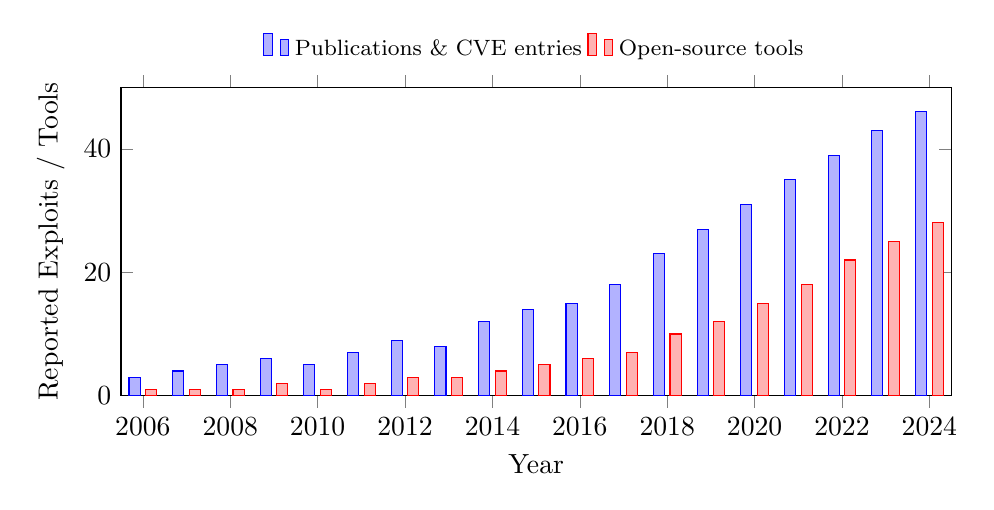
\begin{tikzpicture}
\begin{axis}[
    width=\columnwidth,
    height=5.5cm,
    ybar,
    bar width=4pt,
    ymin=0, ymax=50,
    xmin=2005.5, xmax=2024.5,
    xtick={2006,2008,2010,2012,2014,2016,2018,2020,2022,2024},
    xticklabel style={/pgf/number format/1000 sep=},
    ylabel={Reported Exploits / Tools},
    xlabel={Year},
    legend style={at={(0.5,1.05)}, anchor=south, legend columns=2,
                  font=\footnotesize, draw=none},
]
\addplot coordinates {
(2006, 3)(2007, 4)(2008, 5)(2009, 6)(2010, 5)(2011, 7)
(2012, 9)(2013, 8)(2014,12)(2015,14)(2016,15)(2017,18)
(2018,23)(2019,27)(2020,31)(2021,35)(2022,39)(2023,43)(2024,46)
};
\addplot coordinates {
(2006, 1)(2007, 1)(2008, 1)(2009, 2)(2010, 1)(2011, 2)
(2012, 3)(2013, 3)(2014, 4)(2015, 5)(2016, 6)(2017, 7)
(2018,10)(2019,12)(2020,15)(2021,18)(2022,22)(2023,25)(2024,28)
};
\legend{Publications \& CVE entries, Open-source tools}
\end{axis}
\end{tikzpicture}
\captionof{figure}{Growth of documented NFC/RFID exploits and open-source attack tools (2006--2024). Data from peer-reviewed literature and the CVE database.}
\label{fig:threat_growth}
\end{center}

Beyond raw quantity, the diversity of attack vectors has expanded considerably, as summarized in Figure~\ref{fig:attack_taxonomy}. Early threats were largely limited to passive eavesdropping and relay; modern adversaries now employ card emulation, side-channel analysis, algebraic key-recovery, and multi-layer protocol exploitation~\cite{kasper2012all}. The emergence of the ``Chinese Magic Card'' (rewritable Block~0 MIFARE chips) has further commoditised cloning attacks, enabling an attacker to duplicate both the UID and the sector payload without specialist fabrication equipment.

\begin{center}
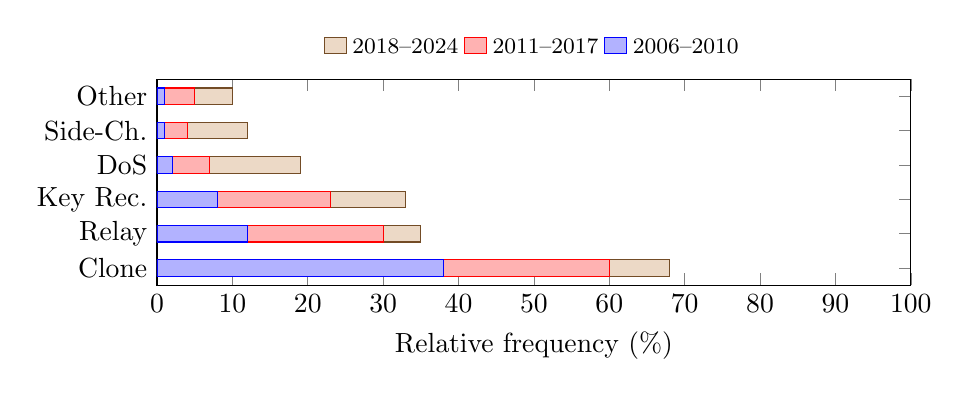
\begin{tikzpicture}
\begin{axis}[
    width=0.92\columnwidth,
    height=4.2cm,
    xbar stacked,
    xmin=0, xmax=100,
    ytick={1,2,3,4,5,6},
    yticklabels={Clone,Relay,Key Rec.,DoS,Side-Ch.,Other},
    xlabel={Relative frequency (\%)},
    legend style={at={(0.5,1.05)}, anchor=south, legend columns=3,
                  font=\footnotesize, draw=none},
    reverse legend,
    bar width=6pt,
]
\addplot coordinates {(38,1)(12,2)(8,3)(2,4)(1,5)(1,6)};
\addplot coordinates {(22,1)(18,2)(15,3)(5,4)(3,5)(4,6)};
\addplot coordinates {(8,1)(5,2)(10,3)(12,4)(8,5)(5,6)};
\legend{2006--2010,2011--2017,2018--2024}
\end{axis}
\end{tikzpicture}
\captionof{figure}{Evolution of NFC attack-vector distribution across three time periods. Cloning and relay remain dominant, but key-recovery and denial-of-service attacks have grown notably since 2018.}
\label{fig:attack_taxonomy}
\end{center}

Beyond raw quantity, the diversity of attack vectors has expanded considerably, as summarized in Figure~\ref{fig:attack_taxonomy}. Early threats were largely limited to passive eavesdropping and relay; modern adversaries now employ card emulation, side-channel analysis, algebraic key-recovery, and multi-layer protocol exploitation~\cite{kasper2012all}. The emergence of the ``Chinese Magic Card'' (rewritable Block~0 MIFARE chips) has further commoditised cloning attacks, enabling an attacker to duplicate both the UID and the sector payload without specialist fabrication equipment.

The combination of a growing attack surface and commodity-grade offensive hardware has eroded the implicit ``proximity-equals-security'' assumption on which most NFC access-control deployments were originally designed. This motivates the need for defense mechanisms that operate below the protocol layer, at the physical radio interface, where adversarial presence can be detected from signal-level anomalies rather than from credential content alone.

\subsection{Contributions and Paper Organization}

In this work, we investigate NFC smart lock security from both adversarial and defensive perspectives, using openly available hardware and software toolchains. Our principal contributions are as follows:

\begin{enumerate}
\item \textbf{End-to-end attack demonstration.} We replicate a complete credential-recovery and card-cloning attack against MIFARE Classic 1K access cards, leveraging a Proxmark3 platform to exploit the well-documented weaknesses of the Crypto-1 stream cipher. The attack chain covers nonce collection, key recovery, sector dump, and production of a functional clone using rewritable Magic Cards.
\item \textbf{Physical-layer anti-cloning defense.} We propose a defense strategy that operates at the 13.56~MHz RF physical layer, independent of the upper-layer protocol. By capturing reader-card interactions with a HackRF One SDR and analyzing per-card signal fingerprints, we create a verification pipeline that can distinguish a genuine card from an identical clone.
\item \textbf{Integrated prototype system.} We build and release a cross-platform smart lock implementation that combines standard PCSC card I/O with the SDR-based fingerprint verification, serving as a reproducible testbed for both attack and defense evaluation.
\end{enumerate}

The remainder of this paper is organized as follows. Section~2 provides background on MIFARE Classic and the Crypto-1 cipher. Section~3 presents the implementation of our smart lock system. Section~4 analyzes the theoretical weaknesses of the Crypto-1 cipher and their exploitation methodology. Section~5 describes the practical Proxmark3-based attack implementation and experimental results. Section~6 presents the physical-layer fingerprinting defense. Section~7 discusses limitations and future work, and Section~8 concludes.

\section{MIFARE Classic and Crypto-1}
\label{sec:background}

\subsection{MIFARE Classic Memory Architecture}

The MIFARE Classic 1K is one of the most widely deployed contactless smart cards globally, consisting of a chip, antenna, and card body as illustrated in Figure~\ref{fig:insidemifare}.

\begin{figure}[H]
\centering
\begin{tikzpicture}
    \node[anchor=south west, inner sep=0] (image) at (0,0) {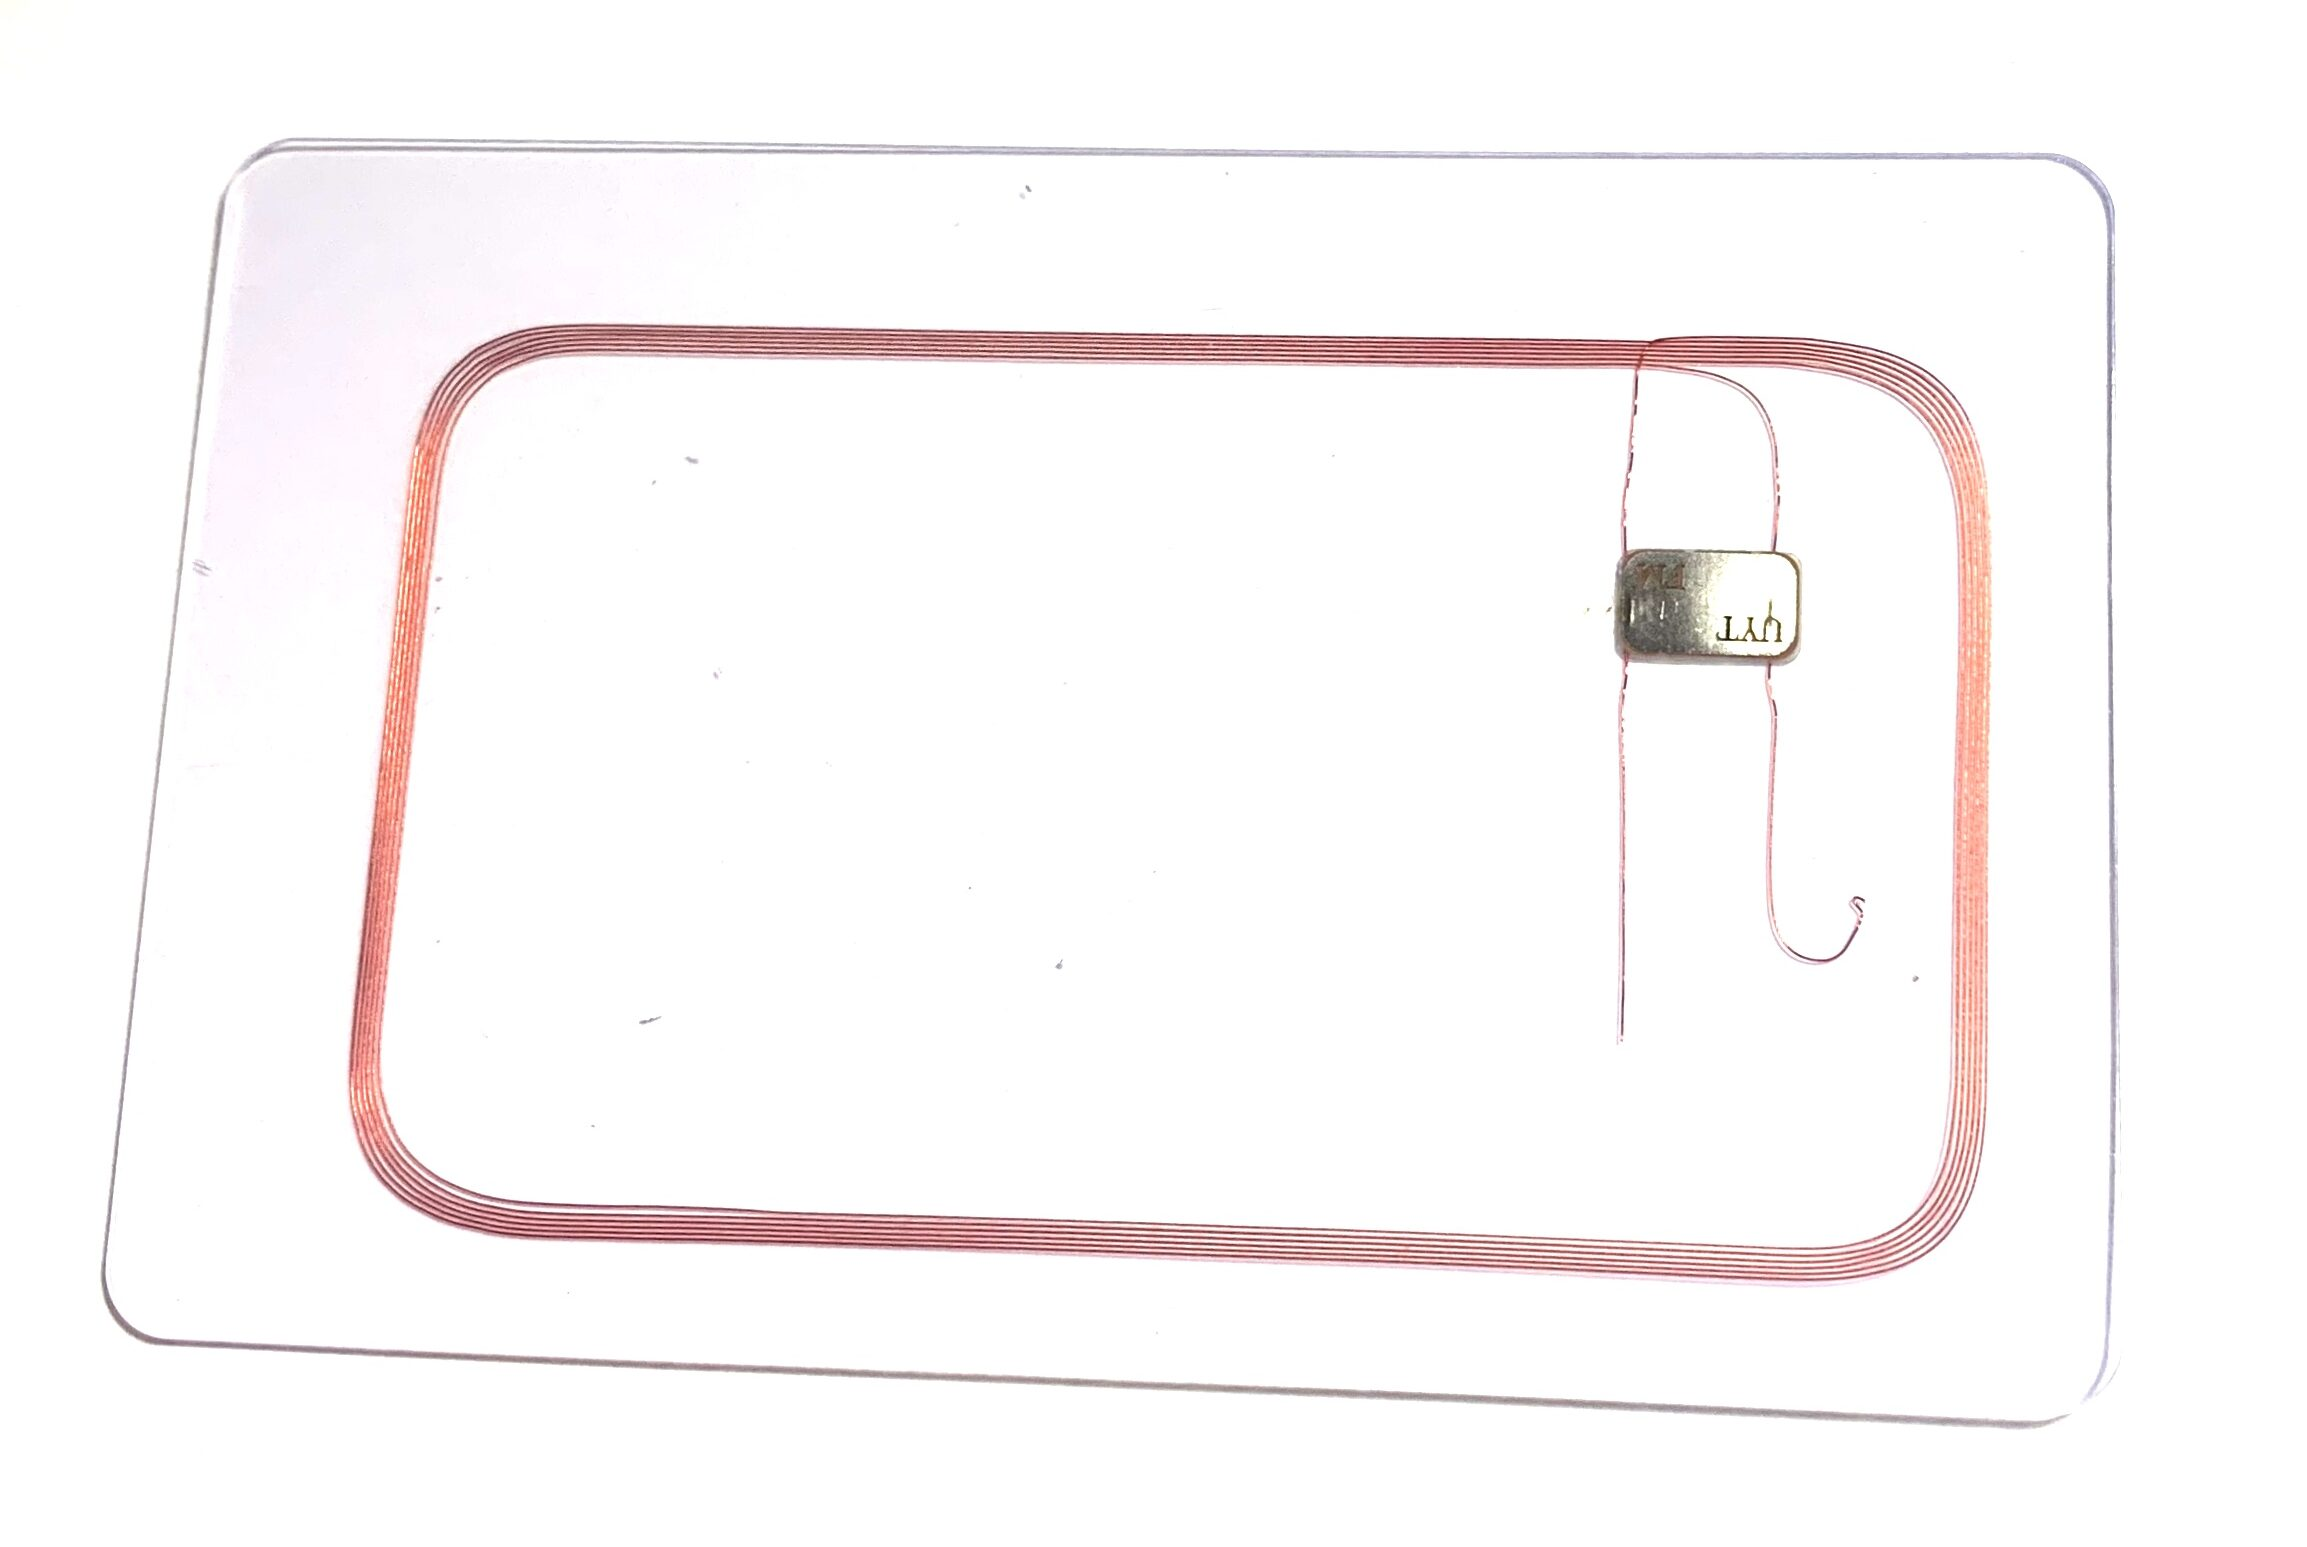
\includegraphics[width=0.9\columnwidth]{insidemifare.jpg}};
    
    \begin{scope}[x={(image.south east)},y={(image.north west)}]        
        \node[text=red, font=\bfseries] (text1) at (0.5, 0.95) {Antenna Coils};
        \draw[-stealth, thick, red] (text1.south) -- (0.5, 0.8);

        \node[text=red, font=\bfseries] (text2) at (0.8, 0.85) {IC Chip};
        \draw[-stealth, thick, red] (text2.south) -- (0.75, 0.65);

    \end{scope}
\end{tikzpicture}
\caption{MIFARE Classic 1K}
\label{fig:insidemifare}
\end{figure}

Operating at 13.56~MHz, it complies with parts 1--3 of the ISO/IEC 14443 Type A standard but diverges at the application layer by employing a proprietary protocol and cryptographic algorithm for access control~\cite{finkenzeller2010rfid}. The 1K variant features 1024 bytes of EEPROM, which is partitioned into 16 discrete sectors (numbered 0 to 15), as illustrated in Figure~\ref{fig:mifare_memory}.

\begin{figure}[H]
\centering
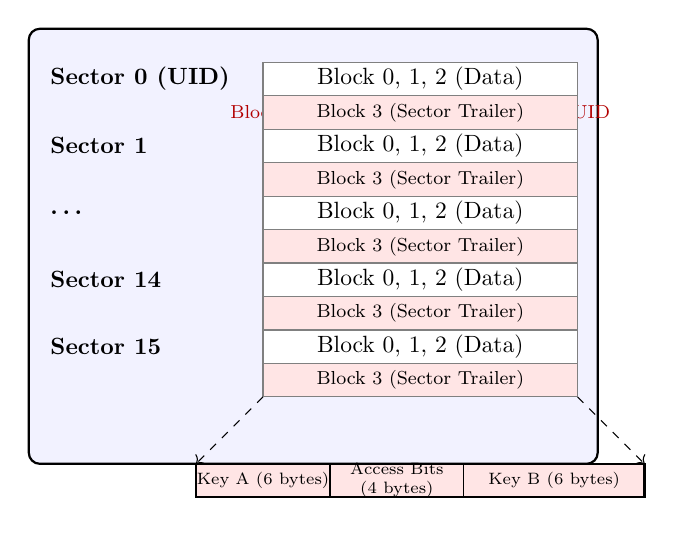
\begin{tikzpicture}[scale=0.85, every node/.style={transform shape}]
    \draw[thick, rounded corners, fill=blue!5] (0, 0) rectangle (8.5, 6.5);
    
    \foreach \y/\sec in {5.5/Sector 0 (UID), 4.5/Sector 1, 3.5/\dots, 2.5/Sector 14, 1.5/Sector 15} {
        \node[anchor=west, font=\bfseries] at (0.2, \y+0.25) {\sec};
        \draw[fill=white, draw=gray] (3.5, \y) rectangle (8.2, \y+0.5);
        \node at (5.85, \y+0.25) {Block 0, 1, 2 (Data)};
        \ifnum\pdfstrcmp{\sec}{Sector 0 (UID)}=0
            \node[font=\footnotesize, color=red!70!black] at (5.85, \y) [below] {Block 0 contains Manufacturer Data / UID};
        \fi
        \draw[fill=red!10, draw=gray] (3.5, \y-0.5) rectangle (8.2, \y);
        \node[font=\footnotesize] at (5.85, \y-0.25) {Block 3 (Sector Trailer)};
    }
    
    \draw[dashed, ->] (3.5, 1) -- (2.5, 0);
    \draw[dashed, ->] (8.2, 1) -- (9.2, 0);
    \draw[fill=red!10, thick] (2.5, -0.5) rectangle (9.2, 0);
    \draw (4.5, -0.5) -- (4.5, 0);
    \draw (6.5, -0.5) -- (6.5, 0);
    
    \node[font=\scriptsize] at (3.5, -0.25) {Key A (6 bytes)};
    \node[font=\scriptsize, align=center] at (5.5, -0.25) {Access Bits\\(4 bytes)};
    \node[font=\scriptsize] at (7.85, -0.25) {Key B (6 bytes)};
\end{tikzpicture}
\caption{MIFARE Classic 1K memory organization and Sector Trailer structure.}
\label{fig:mifare_memory}
\end{figure}

Each sector consists of four 16-byte blocks. The first three blocks (Blocks 0--2) are allocated for user data storage. A notable exception is Block 0 of Sector 0, which is programmed during silicon manufacturing and contains the 4-byte or 7-byte Unique Identifier (UID) alongside vendor data. By design, this block is permanently write-protected on authentic tags. The final block of every sector, known as the Sector Trailer (Block 3), dictates the access control policies for that specific sector. It holds two 48-bit authentication keys (Key A and Key B) separated by four bytes of access conditions. These conditions define the read and write permissions for the data blocks and the sector trailer itself, dependent on which key is successfully authenticated.

\subsection{The Crypto-1 Stream Cipher}

To protect data transmission and enforce sector-level access control, NXP Semiconductors implemented Crypto-1, a proprietary stream cipher. The algorithm's design was kept secret under the premise of security through obscurity until it was successfully reverse-engineered by Garcia et al.\ in 2008 through microscopic silicon analysis~\cite{garcia2008dismantling}.

Crypto-1 utilizes a 48-bit Linear Feedback Shift Register (LFSR) combined with a multi-layered non-linear boolean filter function $f(x)$ (Figure~\ref{fig:crypto1_arch}). The LFSR state is updated at each clock cycle based on a primitive feedback polynomial over GF(2). The generated keystream is subsequently XORed with the plaintext to produce ciphertext during reader-card over-the-air communication.

\begin{figure}[H]
\centering
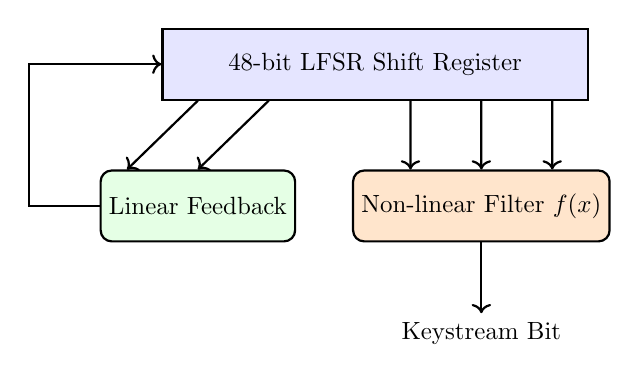
\begin{tikzpicture}[scale=0.9, every node/.style={transform shape}]
    \node[draw, thick, fill=blue!10, minimum width=6cm, minimum height=1cm] (lfsr) at (0, 2) {48-bit LFSR Shift Register};
    \node[draw, thick, fill=orange!20, rounded corners, minimum width=3cm, minimum height=1cm] (filter) at (1.5, 0) {Non-linear Filter $f(x)$};
    \node[draw, thick, fill=green!10, rounded corners, minimum width=2cm, minimum height=1cm] (feedback) at (-2.5, 0) {Linear Feedback};
    
    \draw[->, thick] ([xshift=1.5cm]lfsr.south) -- (filter.north);
    \draw[->, thick] ([xshift=0.5cm]lfsr.south) -- ([xshift=-1cm]filter.north);
    \draw[->, thick] ([xshift=2.5cm]lfsr.south) -- ([xshift=1cm]filter.north);
    
    \draw[->, thick] (filter.south) -- +(0, -1) node[below] {Keystream Bit};
    
    \draw[->, thick] ([xshift=-1.5cm]lfsr.south) -- (feedback.north);
    \draw[->, thick] ([xshift=-2.5cm]lfsr.south) -- ([xshift=-1cm]feedback.north);
    
    \draw[->, thick] (feedback.west) -- +(-1, 0) |- (lfsr.west);
\end{tikzpicture}
\caption{High-level architecture of the Crypto-1 stream cipher.}
\label{fig:crypto1_arch}
\end{figure}

The sector authentication process relies on a three-pass mutual authentication protocol:
\begin{enumerate}
    \item \textbf{Challenge:} The reader requests authentication for a specific sector block, and the card responds with a 32-bit random nonce ($n_T$).
    \item \textbf{Response \& Reader Nonce:} The reader responds with its own 32-bit nonce ($n_R$) and the encrypted answer to the card's challenge, computed using the shared 48-bit sector key and the initial LFSR state.
    \item \textbf{Card Verification:} If the reader's response is correct, the card replies with the encrypted answer to the reader's challenge, concluding the cryptographic handshake.
\end{enumerate}

Despite its efficiency in resource-constrained environments, Crypto-1 exhibits several critical cryptographic flaws. The 48-bit key space is susceptible to brute-force attacks on modern hardware. More importantly, the reliance on a predictable pseudo-random number generator (PRNG) for generating $n_T$ and the malleability of the parity bits in the ISO 14443-A framing allow attackers to deduce the internal LFSR state. Section~\ref{sec:attack-theory} examines the cryptanalytic theory behind these weaknesses, while Section~\ref{sec:attack-practice} demonstrates their practical exploitation with a Proxmark3.

\section{Smart Lock System Implementation}
\label{sec:White part}

为了展开后续的攻防实践，我们在此基于上述的 MIFARE Classic 1K 卡片的交互原理、Crypto-1 加密算法及相关的 NFC 通信协议，使用 C 语言构建了一款可用于与加密卡交互的智能门锁系统。目前，该系统的核心功能为根据读取的信息验证身份，并决定是否发出开锁信号。因此，其他人可根据源码预留的接口驱动其他门锁组件进行实际的开关锁操作。

\subsection{System Architecture}

智能门锁系统的总体架构由三个逻辑层次构成，如图~\ref{fig:lock_arch} 所示：最顶层为运行于宿主机上的锁守护进程（\texttt{lock}）和卡片管理工具（\texttt{lock\_admin}），中间层为操作系统的 PC/SC 智能卡框架，最底层为通过 USB CCID 接口连接的 ACR122U NFC 读写器及被感应的 MIFARE Classic 1K 门禁卡。

\begin{figure}[htbp]
\centering
\definecolor{codebg}{RGB}{225, 235, 245}
\definecolor{codebd}{RGB}{70, 130, 180}
\definecolor{filebg}{RGB}{255, 248, 220}
\definecolor{apibg}{RGB}{232, 238, 242}
\definecolor{apibd}{RGB}{90, 110, 130}
\definecolor{apibgl}{RGB}{224, 232, 238}
\definecolor{hwbg}{RGB}{245, 232, 230}
\definecolor{hwbd}{RGB}{190, 85, 85}
\definecolor{hwbgl}{RGB}{248, 238, 235}

\begin{tikzpicture}[
    >=Stealth,
    font=\small\sffamily,
    lblk/.style={draw, rounded corners=2pt, align=center, inner sep=2pt,
                 minimum height=0.55cm, font=\scriptsize\ttfamily},
    code/.style={lblk, fill=codebg, draw=codebd},
    fkey/.style={lblk, fill=filebg, draw=orange!70!black},
    bigbox/.style={draw, rounded corners=3pt, align=center, inner sep=2.5pt,
                   font=\scriptsize\sffamily},
    layer/.style={draw, rounded corners=4pt, inner sep=4pt, line width=0.6pt},
    arr/.style={->, line width=0.8pt, draw=black!60},
    darr/.style={<->, line width=0.8pt, draw=hwbd, dashed},
]

\node[layer, fill=blue!6, draw=codebd, minimum width=\columnwidth-0.2cm, minimum height=2.5cm] (L1) at (0, 0) {};
\node[font=\scriptsize\bfseries, anchor=north west] at (L1.north west) {\;C Application Layer};

\node[code, font=\bfseries\footnotesize\ttfamily] (main)   at (0,    0.7)  {main.c};
\node[code] (admin)  at (-3.0, 0.7)  {admin.c};
\node[code] (hw)     at (2.5,  0.7)  {hardware\_ctrl.c};
\node[code] (crypto) at (-3.0, -0.1) {crypto\_engine.c};
\node[code] (readin) at (2.5,  -0.1) {readin.c};
\node[fkey] (keys)   at (-0.5, -0.1) {keys.txt\\[-1pt]\tiny (白名单)};

\node[layer, fill=apibgl, draw=apibd, minimum width=\columnwidth-0.2cm, minimum height=1.7cm, below=0.55cm of L1] (L2) {};
\node[font=\scriptsize\bfseries, anchor=north west] at (L2.north west) {\;PC/SC Middleware};

\node[bigbox, fill=apibg, draw=apibd, minimum width=\columnwidth-0.8cm] (api) at ($(L2.north)+(0,-0.52)$) {PC/SC API (WinSCard / PCSC-Lite)};
\node[lblk, fill=white, draw=apibd!50, font=\tiny\sffamily] (os1) at ($(L2.south)+(-2.3,0.32)$) {macOS: PCSC.framework};
\node[lblk, fill=white, draw=apibd!50, font=\tiny\sffamily] (os2) at ($(L2.south)+(0,0.32)$)    {Linux: pcsc-lite};
\node[lblk, fill=white, draw=apibd!50, font=\tiny\sffamily] (os3) at ($(L2.south)+(2.3,0.32)$)  {Windows: WinSCard};

\node[layer, fill=hwbgl, draw=hwbd, minimum width=\columnwidth-0.2cm, minimum height=1.5cm, below=0.55cm of L2] (L3) {};
\node[font=\scriptsize\bfseries, anchor=north west] at (L3.north west) {\;Hardware Layer};

\node[bigbox, fill=hwbg, draw=hwbd, minimum width=2.5cm] (reader) at ($(L3.center)+(-1.8, -0.05)$) {ACR122U\\NFC读写器\\[-1pt]\tiny(USB CCID)};
\node[bigbox, fill=hwbg, draw=hwbd, minimum width=2.5cm] (card)   at ($(L3.center)+(1.8, -0.05)$)  {MIFARE Classic 1K\\门禁卡\\[-1pt]\tiny(ISO 14443-A)};

\draw[arr] (readin.south) -- ++(0, -0.75) -| (L2.north)
    node[pos=0.5, above, xshift=1.2cm, font=\tiny] {APDU / SCard API};
\draw[arr] (L2.south) -- ++(0, -0.45) -| (reader.north)
    node[pos=0.5, above, xshift=1.0cm, font=\tiny] {USB CCID};

\draw[->, gray, thick] (main.west) -- (admin.east);
\draw[->, gray, thick] (main.east) -- (hw.west);
\draw[->, gray, thick] (admin.south) -- (crypto.north);
\draw[->, gray, thick] (hw.south) -- (readin.north);
\draw[->, gray, thick] (crypto.east) -- (keys.west);

\draw[darr] (reader.east) -- (card.west) node[midway, above, font=\tiny\bfseries] {13.56 MHz};

\end{tikzpicture}
\caption{智能门锁系统三层架构。}
\label{fig:lock_arch}
\end{figure}


系统被构建为两个独立的可执行文件（共享同一代码库），分别承担不同的角色：
\begin{itemize}
    \item \texttt{lock}——门锁守护进程。以无限循环方式运行，不断等待卡片靠近、执行身份验证、根据验证结果控制 LED 灯信号和蜂鸣器提示，并记录访问事件。
    \item \texttt{lock\_admin}——卡片发行与管理工具。用于将凭证数据（加密密钥、访问等级、有效期等）写入空白卡片，完成卡片初始化与注册。
\end{itemize}

系统的核心代码组织在 \texttt{src/} 目录下，结构如下：

\texttt{main.c}（224 行）是锁守护进程的入口点。它首先解析命令行参数（\texttt{-{}-keyfile} 指定白名单文件路径，\texttt{-{}-keya} 可选自定义 Key A），安装操作系统信号处理器（SIGINT、SIGTERM、SIGHUP）以保证退出时释放 PC/SC 资源，然后初始化 PC/SC 上下文并自动选择名中包含 ``ACR122'' 或 ``ACR12'' 的读卡器。之后进入无限主循环：等待卡片靠近 $\to$ 连接卡片 $\to$ 调用 \texttt{auth\_verify\_card()} 验证凭证 $\to$ 根据返回值控制 LED 信号 $\to$ 断开连接 $\to$ 等待卡片移走，循环往复。

\texttt{admin.c}（331 行）是管理工具 \texttt{lock\_admin} 的实现。通过参数 \texttt{-{}-level} 设置访问等级、\texttt{-{}-expiry} 设置有效期（BCD 编码）、\texttt{-{}-keya} 设置自定义密钥、\texttt{-{}-format-trailer} 控制是否格式化扇区尾块。程序在用户放置卡片并按回车后执行写卡操作：将凭证头写入 Block~4、随机生成的 8 字节凭证密钥写入 Block~5、发行日期和有效期写入 Block~6，并进行写后回读验证。凭证密钥由标准库 \texttt{rand()} 生成。

\texttt{crypto\_engine.c}（599 行）是整个系统最关键的模块，封装了所有 MIFARE Classic 卡片的密码学操作。主要函数包括：
\begin{itemize}
    \item \texttt{apdu\_send()} / \texttt{apdu\_ok()}——APDU 指令的发送与应答校验
    \item \texttt{mifare\_load\_key()}——向 ACR122U 密钥槽加载 Key A
    \item \texttt{mifare\_authenticate()}——执行三次相互认证
    \item \texttt{mifare\_read\_block()} / \texttt{mifare\_write\_block()}——加密会话下的数据块读写
    \item \texttt{auth\_verify\_card()}——凭证全链路验证（详见 \S\ref{subsec:auth_flow}）
    \item \texttt{load\_whitelist()} / \texttt{is\_in\_whitelist()}——白名单加载与匹配
\end{itemize}

\texttt{readin.c}（113 行）提供 PC/SC 的跨平台抽象层，封装了上下文建立、读卡器枚举、卡片连接/断开、等待卡片到位/移走等操作。所有底层 API 差异（macOS 的 \texttt{PCSC.framework}、Linux 的 \texttt{libpcsclite}、Windows 的 \texttt{WinSCard}）由条件编译统一处理。

\texttt{hardware\_ctrl.c}（64 行）实现 LED 灯和蜂鸣器的硬件控制。ACR122U 的 LED/蜂鸣器通过厂商特定 APDU 指令（CLA \texttt{0xFF}，INS \texttt{0x40}）进行控制：验证通过时发送绿色 LED 闪烁（状态 \texttt{0x08}，500ms 间隔），验证失败时发送红色 LED 闪烁（状态 \texttt{0x04}，200ms 间隔）三次。

\subsection{Hardware Components}

本系统的硬件组成遵循典型的商用智能门锁方案架构。核心硬件包括三个部分：NFC 读写器、门禁卡片和宿主机。

\subsubsection{ACR122U NFC 读写器}

ACR122U（及兼容型号如 ACR122T）是 Advanced Card Systems Ltd.（ACS）生产的一款符合 CCID 标准的非接触式智能卡读写器，作为本系统的门端读卡装置。它通过 USB 全速接口（12~Mbps）与宿主机通信，遵循 USB CCID 设备类规范，操作系统无需安装专有驱动即可通过标准 PC/SC 框架进行访问。

\begin{figure}[H]
\centering
\begin{tikzpicture}
    \node[anchor=south west, inner sep=0] (image) at (0,0) {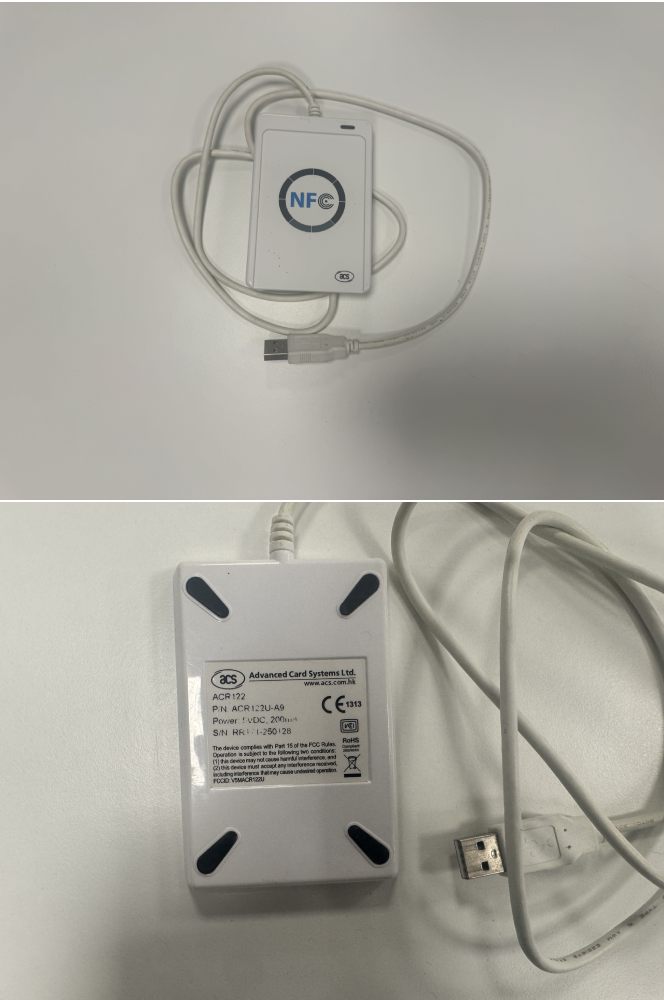
\includegraphics[width=0.85\columnwidth]{ACR122U.png}};
    \begin{scope}[x={(image.south east)},y={(image.north west)}]
        \node[text=black, font=\footnotesize\sffamily] (label1) at (0.05, 0.55) {Front};
        \node[text=black, font=\footnotesize\sffamily] (label2) at (0.05, 0.45) {Back};
    \end{scope}
\end{tikzpicture}
\caption{ACR122U}
\label{fig:acr122u}
\end{figure}

该读写器的核心射频组件工作于 13.56 MHz，兼容 ISO/IEC 14443 Type A 和 Type B 协议。对于 MIFARE Classic 卡片，ACR122U 在固件中集成了 Crypto-1 硬件引擎，能够在设备内部完成三次相互认证的密码学运算。这意味着上位机端的软件仅需通过 APDU 指令向读写器发送 Key A（\texttt{FF 82 00 00 06 <key>}）和认证命令（\texttt{FF 86 00 00 05 01 00 <block> 60 00}），即可获取认证成功/失败的状态码——原始的非交互挑战/应答序列（$n_T$、$n_R$、$a_R$、$a_T$）在上位机侧不可见，加密和解密过程完全在读写器内部完成。这一特性简化了上位机软件开发，但也意味着若要嗅探原始 RF 信号或捕获认证序列，必须借助 Proxmark3 等专用工具在物理层旁路监听。

读写器内置可编程的双色 LED 灯（红/绿）和蜂鸣器。本系统通过厂商自定义 APDU \texttt{FF 00 40} 直接控制它们，以实现访问授权/拒绝的视觉反馈。LED 控制指令通过 P2 参数区分状态：\texttt{0x08} 对应绿色 LED 闪烁，\texttt{0x0C} 对应关闭 LED，\texttt{0x04} 对应红色 LED 闪烁。闪烁的占空比由发送指令的时间间隔控制（验证通过时 500ms，拒绝时 200ms）。

\subsubsection{MIFARE Classic 1K 门禁卡片}

系统使用 NXP 半导体生产的 MIFARE Classic 1K（S50）作为用户门禁卡。该卡片的具体内存布局和加密特性已在第~\ref{sec:background} 节中详细描述，此处仅从门锁系统的应用角度说明凭证数据的组织方式。

系统使用了卡片的 Sector 1（Block 4--7，即第二个扇区）来存储门禁凭证。Sector 0 保留给制造商的 UID 和出厂数据，Sectors 2--15 在本系统不使用。Sector 1 中各块的用途如表~\ref{tab:credential_layout} 所示。

\begin{table}[H]
\centering
\caption{Sector 1 凭证数据布局}
\label{tab:credential_layout}
\begin{tabular}{@{}clp{5cm}@{}}
\toprule
\textbf{块号} & \textbf{名称} & \textbf{内容} \\
\midrule
Block 4 & 凭证头 & 魔术字符串 \texttt{"LOCK"}（4 字节）+ 卡片序列号（4 字节）+ 访问等级（2 字节）+ 保留（6 字节）\\
Block 5 & 凭证密钥 & 随机生成的 8 字节凭证密钥 + 保留（8 字节）\\
Block 6 & 元数据 & 发行日期 BCD（4 字节）+ 有效期 BCD（4 字节）+ 保留（8 字节）\\
Block 7 & 扇区尾块 & Key A（6 字节）+ 访问条件（4 字节）+ Key B（6 字节）\\
\bottomrule
\end{tabular}
\end{table}

凭证头的魔术字符串 \texttt{"LOCK"} 用于识别该卡片是否为本系统发放的门禁卡。卡片序列号字段存储了卡片物理 UID 的前 4 字节，在每次验证时与实际卡片 UID 进行比对，作为反克隆的基础措施。凭证密钥为 \texttt{lock\_admin} 发行时随机生成的 8 字节密钥，在宿主机的白名单文件 \texttt{keys.txt} 中注册，构成离线白名单访问控制系统。有效期采用 BCD 编码（例如 2026 年 12 月 31 日表示为字节序列 \texttt{0x20 0x26 0x12 0x31}），由系统时钟在每次验证时进行比对检查。

系统默认使用出厂密钥 \texttt{FF FF FF FF FF FF} 作为 Sector 1 的 Key A，可在运行时通过 \texttt{-{}-keya} 参数指定自定义密钥。访问条件（默认为 \texttt{FF 07 80 69}）编码为 Key A 不可读（仅可写），Key B 可读写，由 Key A 认证后可读取所有数据块但不能写入。该策略确保了门锁守护进程仅需知道 Key A 即能完成验证，管理工具需要 Key A 进行写卡操作，而卡片内容不会被非授权方轻易读出。

\subsection{Authentication and Verification Pipeline}
\label{subsec:auth_flow}

一次完整的卡片认证与验证流程，从卡片靠近到门锁决策，共经历以下七个阶段。该流程由 \texttt{crypto\_engine.c} 中的 \texttt{auth\_verify\_card()} 函数统一协调。

\textbf{阶段 1：卡片到位检测。} 守护进程通过 \texttt{pcsc\_wait\_for\_card()} 阻塞等待读卡器报告卡片就位。该函数内部使用 \texttt{SCardGetStatusChange()} 轮询读卡器状态，当状态字中的 \texttt{SCARD\_STATE\_PRESENT} 位被置位时返回。

\textbf{阶段 2：建立连接与读取 UID。} 调用 \texttt{SCardConnect()} 以共享模式（\texttt{SCARD\_SHARE\_SHARED}）连接卡片，同时协商传输协议（T=0 或 T=1）。随后通过 APDU \texttt{FF CA 00 00 00}（Get Data）读取卡片的物理 UID。UID 长度为 4 或 7 字节（MIFARE Classic 1K 通常为 4 字节），提取前 4 字节用于后续与存储序列号的比对。

\textbf{阶段 3：加载密钥与三次相互认证。} 通过 APDU \texttt{FF 82 00 00 06 <Key A>} 将 Sector 1 的 Key A 加载到 ACR122U 的易失性密钥槽中。随后发送认证指令 \texttt{FF 86 00 00 05 01 00 04 60 00}，指示读写器对 Block 4（Sector 1 的第一个数据块）执行 Crypto-1 三次相互认证。此认证由 ACR122U 内部硬件引擎完成，主控端仅收到成功（SW=\texttt{90 00}）或失败（SW=\texttt{63 Cx}，其中 \texttt{x} 为剩余重试次数）的状态码。

\textbf{阶段 4：凭证头验证。} 认证通过后，加密会话已建立。通过 APDU \texttt{FF B0 00 04 10} 读取 Block 4 的 16 字节完整内容。首先检查前 4 字节是否等于魔术字符串 \texttt{"LOCK"}，以确认该卡片为本系统发放的门禁卡。然后提取 Block 4 中存储的 4 字节序列号（偏移 4--7），与阶段 2 中读取的物理 UID 前 4 字节进行比对。两者不一致则拒绝访问（返回 \texttt{AUTH\_FAIL\_UID}），此项检查用于防止将凭证数据复制到另一张物理卡片（若要绕过此项检查，攻击者需使用可修改 UID 的 ``Chinese Magic Card''）。

\textbf{阶段 5：白名单匹配。} 通过 APDU \texttt{FF B0 00 05 10} 读取 Block 5 的前 8 字节（凭证密钥）。在此之前，白名单文件 \texttt{keys.txt} 已被加载到内存（最大支持 64 条记录），每条记录为 16 个十六进制字符表示的 8 字节密钥。通过逐字节比较（\texttt{memcmp}）检查卡片上的凭证密钥是否存在于白名单中。不存在则返回 \texttt{AUTH\_FAIL\_NOT\_IN\_LIST}。白名单文件以 \texttt{\#} 开头的行为注释，支持运行时通过重载信号（SIGHUP）重新加载，实现无停机的用户权限管理。

\textbf{阶段 6：有效期检查。} 通过 APDU \texttt{FF B0 00 06 10} 读取 Block 6 中的 4 字节有效期 BCD。与当前系统日期（\texttt{localtime()}）比较：若已过期则返回 \texttt{AUTH\_FAIL\_EXPIRED}，有效期为 0 表示永不过期，\texttt{29991231} 为默认的永不过期值。同时校验发行日期的 BCD 编码合法性，格式异常返回 \texttt{AUTH\_FAIL\_FORMAT}。

\textbf{阶段 7：决策与硬件信号。} 上述全部检查通过后，\texttt{auth\_verify\_card()} 返回 \texttt{AUTH\_SUCCESS}（0）。守护进程根据返回值分别调用不同的硬件信号函数：
\begin{itemize}
    \item 成功：调用 \texttt{hw\_access\_granted()}，发送绿色 LED 闪烁指令（APDU \texttt{FF 00 40 08 04 D0 07 00 00}），持续 500ms 后关闭 LED。
    \item 失败：调用 \texttt{hw\_access\_denied()}，发送红色 LED 闪烁指令三次（每次 200ms 亮、200ms 灭）。
\end{itemize}
随后，守护进程以保留供电状态（\texttt{SCARD\_LEAVE\_CARD}）断开卡片连接，等待 2000ms 让用户移开卡片，然后回到阶段 1，开始下一周期的检测。

\begin{figure}[H]
\centering
\begin{tikzpicture}[
    >=Stealth,
    node distance=0.35cm,
    stage/.style={
        draw, rectangle, rounded corners=2pt, align=left,
        fill=blue!5, draw=blue!40!black,
        minimum width=4.5cm, minimum height=0.75cm,
        inner sep=4pt, font=\footnotesize\sffamily, line width=0.6pt
    },
    arrow/.style={->, line width=0.8pt, draw=black!60},
    result/.style={draw, rectangle, rounded corners=3pt, align=center,
                   minimum width=1.8cm, minimum height=0.7cm,
                   font=\small\bfseries\sffamily, line width=0.8pt},
    annt/.style={font=\tiny\ttfamily, text=black!60},
]
\node[stage] (s1) {1. 卡片到位检测\\\hspace{1em}\scriptsize\texttt{pcsc\_wait\_for\_card()}};
\node[stage, below=of s1] (s2) {2. 连接卡片并读取 UID\\\hspace{1em}\scriptsize APDU \texttt{FF CA 00 00 00}};
\node[stage, below=of s2] (s3) {3. 加载 Key A \& 三次相互认证\\\hspace{1em}\scriptsize APDU \texttt{FF 82} / \texttt{FF 86} (Crypto-1)};
\node[stage, below=of s3] (s4) {4. 凭证头验证\\\hspace{1em}\scriptsize 读 Block~4，校验\texttt{"LOCK"}和 UID};
\node[stage, below=of s4] (s5) {5. 白名单匹配\\\hspace{1em}\scriptsize 读 Block~5，查找\texttt{keys.txt}};
\node[stage, below=of s5] (s6) {6. 有效期检查\\\hspace{1em}\scriptsize 读 Block~6，比较系统日期};
\node[stage, below=of s6] (s7) {7. 硬件信号输出\\\hspace{1em}\scriptsize 控制 ACR122U LED / 蜂鸣器};

\coordinate (spine) at ([xshift=1.2cm]s4.east);

\node[result, fill=red!15, draw=red!60!black, anchor=north] (failbox) at ($(s7.south -| spine) - (0, 0.8)$) {拒绝\\[-2pt]\footnotesize\color{red!70!black}AUTH\_FAIL};
\node[result, fill=green!15, draw=green!50!black, below=0.8cm of s7] (passbox) {授权\\[-2pt]\footnotesize\color{green!50!black}AUTH\_SUCCESS};

\draw[arrow] (s1.south) -- (s2.north);
\draw[arrow] (s2.south) -- (s3.north);
\draw[arrow] (s3.south) -- (s4.north);
\draw[arrow] (s4.south) -- (s5.north);
\draw[arrow] (s5.south) -- (s6.north);
\draw[arrow] (s6.south) -- (s7.north);

\coordinate (spine) at ([xshift=1.2cm]s4.east);
\draw[dashed, red!60!black, line width=0.6pt] (s1.east) -- (s1.east -| spine);
\draw[dashed, red!60!black, line width=0.6pt] (s2.east) -- (s2.east -| spine);
\draw[dashed, red!60!black, line width=0.6pt] (s3.east) -- (s3.east -| spine);
\draw[dashed, red!60!black, line width=0.6pt] (s4.east) -- (s4.east -| spine);
\draw[dashed, red!60!black, line width=0.6pt] (s5.east) -- (s5.east -| spine);
\draw[dashed, red!60!black, line width=0.6pt] (s6.east) -- (s6.east -| spine);
\draw[dashed, red!60!black, line width=0.6pt] (s7.east) -- (s7.east -| spine);
\draw[->, red!60!black, line width=1.0pt] (s1.east -| spine) -- (failbox.north);

\draw[arrow, draw=green!60!black] (s7.south) -- (passbox.north)
    node[midway, right, font=\footnotesize, text=green!50!black, xshift=0.3cm] {全部通过};

\end{tikzpicture}
\caption{智能门锁认证与验证七阶段流程。阶段之间以实线箭头连接表示正常流转；任一阶段验证失败均以红色虚线箭头导向「拒绝」框，全部通过后以绿色箭头导向「授权」框。}
\label{fig:auth_flow}
\end{figure}

\subsection{Administrative Provisioning}

卡片发行与管理由 \texttt{lock\_admin} 工具完成。其工作流程为：

\begin{enumerate}
    \item 用户通过命令行参数指定访问等级、有效期、自定义 Key A 等配置。
    \item 程序通过 PC/SC 建立读写器上下文，等待用户放置空白卡片并按回车确认。
    \item 使用 Key A 对 Sector 1 进行认证，若认证失败则尝试以出厂默认密钥 \texttt{FF FF FF FF FF FF} 重试。
    \item 依次写入 Block 4（凭证头，包含自动获取的卡片 UID）、Block 5（随机生成的 8 字节凭证密钥）、Block 6（当前日期为发行日、参数指定有效期为到期日）。
    \item 每个块的写入均执行回读验证，确保数据写入正确。写入失败或回读不一致时返回相应错误码。
    \item 若指定了 \texttt{-{}-format-trailer} 标志，程序还将写入 Sector 1 的 Block 7（扇区尾块），设置自定义 Key A 和安全的访问条件。由于写入扇区尾块的操作不可逆（一旦写入错误的访问位可能导致卡片永久锁死），此功能需显式确认。
\end{enumerate}

管理工具成功运行后，将新生成的 8 字节凭证密钥以十六进制格式打印输出，供管理员添加到白名单文件中。

\subsection{Security Considerations}

从安全分析的视角审视本系统的白方实现，可以识别若干关键安全边界：

\textbf{Card-UID 绑定。} 系统在发行时记录卡片的物理 UID 到 Block 4，并在验证时与实时读取的物理 UID 比较。这一措施使得单纯复制 Sector 1 数据到另一张卡片无法通过验证。然而，该防御可被 ``Chinese Magic Card''（可修改 Block~0 即 UID 的兼容卡片）绕过——攻击者可利用 Proxmark3 同时克隆 UID 和 Sector 1 的全部数据，生成无差别的功能克隆卡。

\textbf{离线白名单模型。} 系统的访问控制采用白名单而非吊销列表模型：凭证密钥只有存在于 \texttt{keys.txt} 中才能通过验证。吊销用户只需删除其密钥并重启守护进程。这一设计的优势是无卡片侧修改需求，缺点是白名单文件成为系统的关键安全资产——该文件被泄露将导致所有卡片被任意克隆（因攻击者可将任意 8 字节密钥写入卡片并追加到白名单中）。

\textbf{Crypto-1 的隐蔽性。} Key A 以明文形式从宿主机发送到 ACR122U 的 APDU 载荷中。在 USB 层面，这不受 Crypto-1 保护，只是在 USB CCID 通道中以明文传输。若攻击者能够在宿主机 USB 层面进行监听（通过软件 keylogger 或 USB 硬件分析仪），即可直接获取 Key A。幸而，在实际部署中，获取 Key A 对于防御层后续介绍的物理层指纹检测仍嫌不足。

\textbf{物理层不可见性。} 本系统以 ACR122U 作为读写器，Crypto-1 运算在读写器内部完成，上位机不接触原始 RF 调制波形。这使得上层软件既无法感知射频物理层异常（如克隆卡与正版卡在副载波调制瞬态、载波频率偏移等特征上的细微差异），也无法利用这些差异进行深度防御。这一局限性正是第~\ref{sec:Blue part} 节引入 HackRF One SDR 辅助物理层指纹检测的根本动机。

\section{Crypto-1 Cryptanalytic Theory}
\label{sec:attack-theory}

\subsection{Cryptanalytic Basis}

Crypto-1 uses a 48-bit internal state. MIFARE Classic applies it in a proprietary mutual authentication protocol. Published analyses show that weaknesses in the cipher, initialization, and nonce generation can permit key recovery and decryption without treating Crypto-1 as an ideal exhaustive-search problem~\cite{garcia2008dismantling,kasper2012all}. MIFARE Classic protects sectors with independent Key~A and Key~B values. Once one valid key is available, nested-family techniques can use authenticated exchanges as a starting point for recovering a target sector key. The hardnested variant implemented by Proxmark3 is intended for cards for which the simpler nested assumptions are hardened.

The command recorded in the repository selects Block~24 with Key~A as the known source and Block~4 Key~A as the target. Since MIFARE Classic 1K sectors contain four blocks, Block~24 is the first block of Sector~6 and Block~4 is the first block of Sector~1. The command-line mapping therefore expresses a cross-sector recovery attempt from a known Sector~6 credential to the Sector~1 credential used by the smart-lock format.

\subsection{Theoretical End-to-End Validation}

An end-to-end validation can separate three questions. First, \emph{key completeness} can be assessed by checking whether the required Key~A/Key~B positions are populated and whether protected blocks can be read. Second, \emph{logical reproduction} can be assessed by acquiring a fresh image from the emulator or destination card and comparing its UID, data blocks, and sector trailers with the source. Third, \emph{application behavior} can be assessed by presenting the genuine card, emulator, persistent reproduction, and an unrelated control to the same reader configuration and recording each smart-lock decision stage.

For the implemented smart-lock format, the most relevant comparison covers the presented UID, Sector~1 Key~A, and Blocks~4--6. A UID-only reproduction cannot demonstrate equivalence because the lock also performs sector authentication and reads the whitelisted credential and dates. Conversely, a successful Proxmark3 write cannot demonstrate application acceptance without observing the reader-side decision. Separating these layers prevents key recovery, memory copying, and lock acceptance from being reported as if they were the same result.

\subsection{Theoretical Limitations}

The workflow is specific to MIFARE Classic and Crypto-1. It should not be transferred directly to other product families that use different authentication protocols and cryptographic designs. Recovery behavior may also differ between MIFARE Classic revisions because nonce behavior influences which recovery strategy is applicable.

Protocol-level equality does not imply physical-layer equality. A Proxmark3 emulator and a rewritable card can reproduce logical identifiers and memory while using different analog front ends, clock sources, load-modulation circuits, and antennas. Such differences provide the theoretical basis for examining physical-layer fingerprints in the following section.

\section{Proxmark3 Attack Implementation}
\label{sec:attack-practice}

\subsection{Repository Command Workflow}

The Chinese-language instruction file under \texttt{rrg\_other/} records the command families in Table~\ref{tab:attack-workflow}. Actual key values and card identifiers are omitted here.

\begin{table}[H]
\centering
\caption{MIFARE Classic command workflow recorded in the repository.}
\label{tab:attack-workflow}
\small
\begin{tabular}{p{0.28\columnwidth}p{0.53\columnwidth}}
\toprule
\textbf{Command} & \textbf{Function} \\
\midrule
\texttt{hf mf chk --dump} & Test the four explicitly listed candidate keys and save discovered keys. \\
\texttt{hf mf hardnested} & Use the recorded source block/key type to recover the target Block~4 Key~A. \\
\texttt{hf mf dump} & Read a MIFARE Classic 1K image using a key file and save it under the selected name. \\
\texttt{hf mf rdbl} & Attempt an authenticated read of one selected block. \\
\texttt{hf mf eload} & Upload a BIN, EML, or JSON dump to Proxmark3 emulator memory. \\
\texttt{hf mf sim --1k} & Present emulator memory as a MIFARE Classic 1K card. \\
\texttt{hf mf cload} & Copy a binary image to a Gen1a Magic Card. \\
\texttt{hf mf restore} & Restore a MIFARE Classic 1K image with the \texttt{--1k} option, using the authenticated-write path identified in the instruction file for Gen2 cards. \\
\texttt{hf mf wipe} & Invoke the Magic-Card wipe operation. \\
\bottomrule
\end{tabular}
\end{table}
\subsubsection{Candidate-Key Testing}

\texttt{hf mf chk --dump} tests the four candidate keys written explicitly in the instruction file. The \texttt{--dump} option stores discovered keys for later commands. This stage should be distinguished from cryptanalytic recovery: a successful check means that a supplied value was already a valid key. Nevertheless, one valid sector key can serve as the known source required by the hardnested command.

The repository file named \texttt{my\_keys.dic.json} is not a plain-text dictionary despite the \texttt{dic} component in its name. Its \texttt{FileType} field identifies it as an \texttt{mfc v2} card image, and it contains card metadata, sector keys, and block data.

\subsubsection{Hardnested Recovery}

The hardnested command separates the known source parameters from the unknown target parameters. In the recorded command, \texttt{--blk 24}, \texttt{-a}, and \texttt{-k} select the source block, Key~A, and its known value. The options \texttt{--tblk 4} and \texttt{--ta} select target Block~4 and target Key~A. This distinction is essential because the block number determines the sector and the key-type flag determines which half of the trailer credential is being recovered.

The Proxmark3 logs contain multiple hardnested invocations with different source and target blocks. They also contain \texttt{hf mf autopwn}, which combines candidate-key checks, available recovery strategies, key-file generation, emulator transfer, and dump generation. Because \texttt{autopwn} is present in the logs rather than the instruction file, it is treated as additional recorded evidence rather than a step written in that file.

\subsubsection{Memory Acquisition}

\texttt{hf mf dump} uses recovered keys to authenticate and read the card blocks. The retained logs show dump operations producing a 1024-byte binary file and a structured JSON file. Three tracked image pairs are present: \texttt{my\_keys.dic}, \texttt{ID\_lyl}, and \texttt{ID\_ypz}. Each JSON image declares \texttt{mfc v2}, contains 64 block entries and 16 sector-key entries, and has a corresponding 1024-byte binary image.

The binary file is the byte-oriented image used by restoration commands, whereas JSON preserves structured metadata and is directly accepted by the emulator-loading command. These artifacts contain decoded card memory rather than time-domain RF samples; their role is protocol-level reproduction, not physical-layer model training.

\subsubsection{Emulation and Persistent Writing}

\texttt{hf mf eload} transfers a saved image into Proxmark3 emulator memory. The simulation command then presents that memory through the high-frequency interface as a MIFARE Classic 1K card. This path is volatile: it uses the Proxmark3 as the card-side device and does not alter a separate physical card.

For persistent copying, the instruction file assigns \texttt{hf mf cload} to Gen1a cards and \texttt{hf mf restore --1k} to Gen2 cards. The distinction matters because Gen1a cards expose a special write path, while the restore command follows authenticated block writing and requires suitable current keys and access conditions.

\subsection{Recorded Proxmark3 Results}

The retained client logs provide the following directly observable results:

\begin{itemize}
\item \texttt{log\_20260721034814.txt} records \texttt{hf mf eload}, an upload of 64 blocks and 1024 bytes, \texttt{Done!}, and a subsequent \texttt{hf mf sim --1k} command.
\item \texttt{log\_20260722031003.txt} records a dump that saved a 1024-byte binary image and a JSON image.
\item The same log records \texttt{hf mf cload} loading a 1024-byte image, copying it to a Gen1a MIFARE Classic 1K card, loading 64 blocks, and returning \texttt{Done!}.
\item A recorded \texttt{hf mf autopwn} run generated binary and JSON dumps and reported an execution time of seven seconds.
\end{itemize}

These observations establish command completion and artifact generation. A \texttt{Done!} response from a card-writing command indicates that the Proxmark3 client completed that operation; it is not, by itself, a measurement of an access-control decision.

\section{Fingerprinting Defense}
\label{sec:Blue part}

\section{Discussion and Future Work}
\label{sec:discussion}



\section{Conclusion}
This project successfully demonstrates the severe security risks associated with static credential exposure over the NFC interface and provides an academic proof-of-concept for dynamic physical-layer defense. 

% --- 参考文献 ---
\begin{thebibliography}{99}
\bibitem{iceman} RfidResearchGroup. (2026). \emph{The Proxmark3 Open-Source Firmware Ecosystem}. GitHub Repository.
\bibitem{iso14443} ISO/IEC 14443. \emph{Identification cards -- Contactless integrated circuit cards -- Proximity cards}.
\bibitem{finkenzeller2010rfid} K.~Finkenzeller. \emph{RFID Handbook: Fundamentals and Applications in Contactless Smart Cards, Radio Frequency Identification and Near-Field Communication}. 3rd ed., Wiley, 2010.
\bibitem{kasper2012all} T.~Kasper, D.~Oswald, and C.~Paar. ``All You Can Eat or How to Break an NFC MIFARE Classic Card.'' In \emph{Black Hat USA}, 2012.
\bibitem{haselsteiner2006nfc} E.~Haselsteiner and K.~Breitfu\ss. ``Security in Near Field Communication (NFC): Strengths and Weaknesses.'' In \emph{Workshop on RFID Security (RFIDSec)}, 2006.
\bibitem{garcia2008dismantling} F.~D.~Garcia, G.~de~Koning~Gans, R.~Muijrers, P.~van~Rossum, R.~Verdonschot, R.~Wiegerinck, and J.~Horizons. ``Dismantling MIFARE Classic.'' In \emph{ESORICS}, 2008.
\end{thebibliography}

\end{document}
